\section{Backend}

Backend, tedy serverová část, je napsána v programovacím jazyce Rust, za využítí 
knihovny Tide, a interaguje
s PostgreSQL databází. Značna část logiky a integrita je řešena skrz omezení ve
schématu databázových tabulek a skrz ručně napsané SQL příkazy. Frontend se serverem
komunikuje pomocí paradigmatu REST API, přes protokol HTTP, přičemž těla požadavků a
odpovědí jsou ve formátu JSON.

\begin{figure}[h!] 
    \centering
    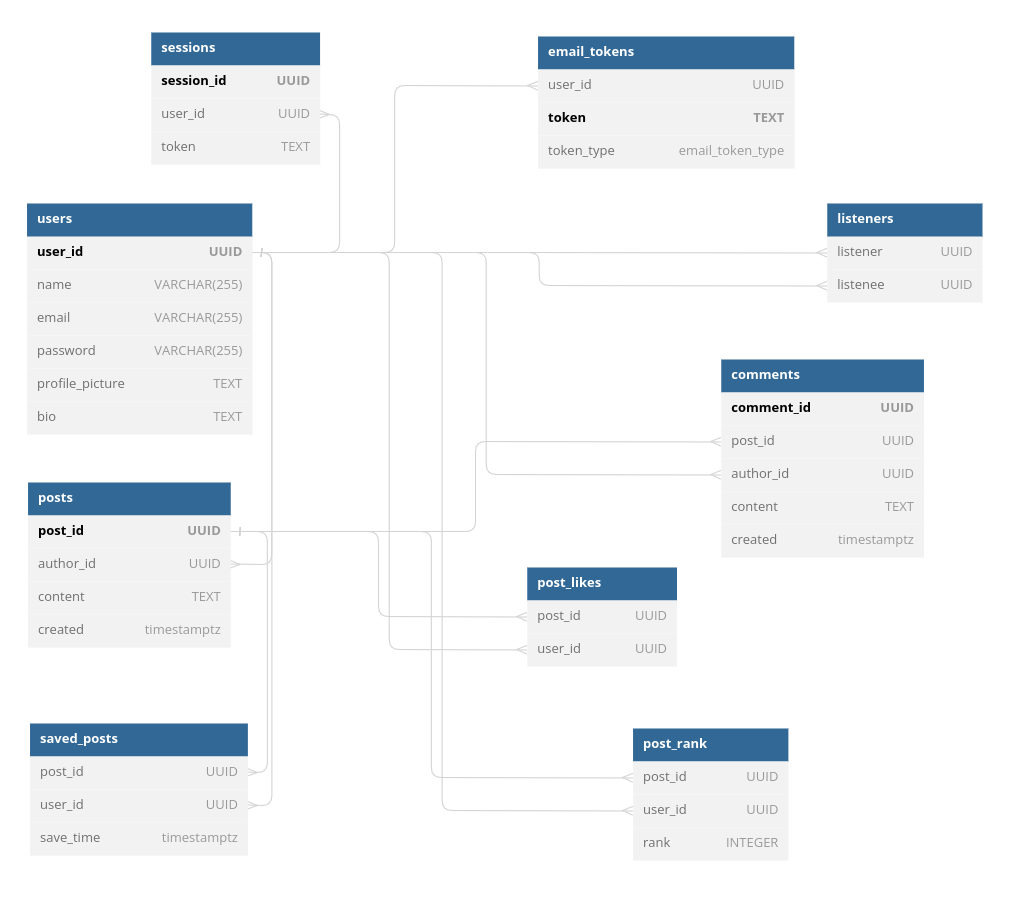
\includegraphics[width=0.8\textwidth]{images/er-diagram.png}
    \caption{ER diagram}
    \label{er-diagram}
\end{figure}

\subsection{Databáze}

Jako databázi jsme zvolili PostgreSQL kvůli rychlosti a množství funkcí, co dokáže.
Celkově má databázové schéma devět tabulek, několik funkcí a náhledů, jak je možno vidět
na obrázku \ref{er-diagram}.

Jedna z výhod PostgreSQL je zabudované full-text vyhledávání, které jsme využili
ve funkci vyhledávání uživatelů. Ve vyhledávání pomocí samotného jména uživatele není
full-text vyhledávání nejlepší metodou, jelikož pracuje s celými slovy, ale velmi se osvědčilo
jako sekundární vyhledávání v celém textu popisku, který si uživatel nastaví.

\subsection{AI rozpoznávání mluvy}

Jeden z hlavních bodů v zadání bylo automatické filtrování mluveného slova. To je možné provést několika
způsoby:

\begin{enumerate}
    \item Analýza frekvencí ve zvukovém souboru.
        \begin{itemize}
            \item Existuje mnoho algoritmu na rozpoznání hlasu, ale ne specificky na mluvené slovo.
            \item Rychlejší, než použití umělé inteligence.
        \end{itemize}
    \item Použití umělé inteligence
        \begin{enumerate}
            \item Využití jednoho z několika veřejných API na rozpoznávání hlasu.
                \begin{itemize}
                    \item Jestliže je nutné API posílat každý příspěvek, pak bude provoz sítě velmi drahý.
                \end{itemize}
            \item Využití již natrénovaného modelu na vlastních strojích.
                \begin{itemize}
                    \item Provozovatel sítě musí mít k dispozici stroje, které dokáží příspěvky rychle zpracovat.
                \end{itemize}
            \item Natrénování vlastního rozpoznávacího modelu a jeho užití na vlastních strojích.
                \begin{itemize}
                    \item Provozovatel musí mít hodně prostředků nejen ke zpracovávání příspěvků, ale také ke trénování modelu.
                \end{itemize}
        \end{enumerate}
\end{enumerate}

Pro Ding jsme zvolili variantu 2. b. Pro rozpoznávání mluveného slova používáme AI model "Whisper AI" od americké
společnosti OpenAI\cite{openai-whisper}. Tento model je veřejně přístupný a je možné si ho spustit na osobním počítači, nebo serveru.
Původní model velmi využívá GPU na grafické kartě počítače. Většina serveru ale grafické karty nemá a tudíž je
nutné výpočty provádět na samotném CPU. Tento problém řeší projekt whisper.cpp od Georgiho Gerganova, který model upravil
tak, aby ho bylo možné spustit na mnohem slabších zařízeních, než jsou speciální počítače OpenAI.

Při přidání nového příspěvku se tedy nejdříve zvukový soubor zkontroluje, že je funkční a ve správném formátu.
Dál se využije AI modelu pro přepsání jakéhokoliv mluveného slova. Pokud je příspěvek v nesprávném formátu, nebo
v něm model najde slova, pak je zpětně smazán. Je tedy možné, že na pár vteřin (nebo minut, záleží na zatížení stroje),
bude příspěvek přístupný, i když by měl být smazán.
